% Author: Joshua Carey

%
\let\textcircled=\pgftextcircled\chapter{Methodology}
% \label{chap:aims_and_opjectives}

% \initial{T}his section will investigate the approach taken to create an autonomous kite-powered vessel.
% - We need a physics engine
% -we need to model a boat so that it behaves with realistic movements
% - need to be able to run machine learning in the physics simulations

% \initial{T}he future of autonomous navigation in maritime settings is not limited to large vessels plying the world's oceans; smaller, nimble crafts, harnessing natural forces such as wind, present their own set of challenges and opportunities. Imagine a vessel, propelled not just by the currents below, but by the gusts above, using a kite to harness the power of the wind. This not only promises sustainable navigation but also offers a glimpse into the intricate dance between machine intelligence, physics, and nature's unpredictability. This project dives deep into simulating such a system— a kite-powered boat that autonomously navigates its environment. This methodology section elucidates the steps taken to bridge the gap between vision and virtual reality.
\initial{T}his project will utilise the Unity game engine as the training environment for RL\@.


\section{MLAgents}
MLAgents is an open-source project that allows games and simulations to serve as the environment for training intelligent agents. At its core MLAgents utilizes RL, although it also supports other methods such as imitation learning.

As discussed in section$~$\ref{RL_background}, RL is an approach to learning where an agent learns to make decisions by interacting with its environment. The fundamental components of this interaction are observations, actions and rewards.
\begin{itemize}
    \item Observations (State): These are the pieces of information that the agent receives from the environment at each step or frame. In Unity, observations are collected through sensors or manually coded to be extracted from the game objects. They are typically fed into the neural network as a vector of floating-point numbers, representing the current state of the environment.
    \item Actions: Based on the observations, the agent takes actions which are the outputs of the neural network. These actions can be discrete (e.g., turn left, turn right) or continuous (e.g., change angle by a certain degree). The neural network's output layer is designed accordingly to provide the appropriate action space for the agent. (Configured as part of the behavioral parameters in Unity)
    \item Rewards: After taking an action, the agent receives a reward signal, which is a numerical value indicating how well the action contributed to achieving its goal. This reward is used to adjust the neural network's weights, with the aim of maximizing the total accumulated reward.
\end{itemize}
A full breakdown of the actions, observations, rewards, and how the agent script configures these for this project can be found in section$~$\ref{sec:RL_Implementation}.


\subsection{Python Implementation}
The neural network used in the reinforcement learning is implemented in Python. MLAgents toolkit is a Python Library that acts as an interface between the Unity game engine and Pytorch [CITE]. PyTorch provides the computational enine that powers the training of neural networks. MLAgents uses a python API to communicate with the Unity environment frame by frame. This stepping process allows for the synchronous collection of observations, executions of actions and retrieval of rewards. The neural network used in this project is a Proximal Policy Optimization (PPO) network, and so will utilise the actor-critic method as discussed in section$~$\ref{sec:ppo_background}.

\begin{figure}[h]
    \centering
    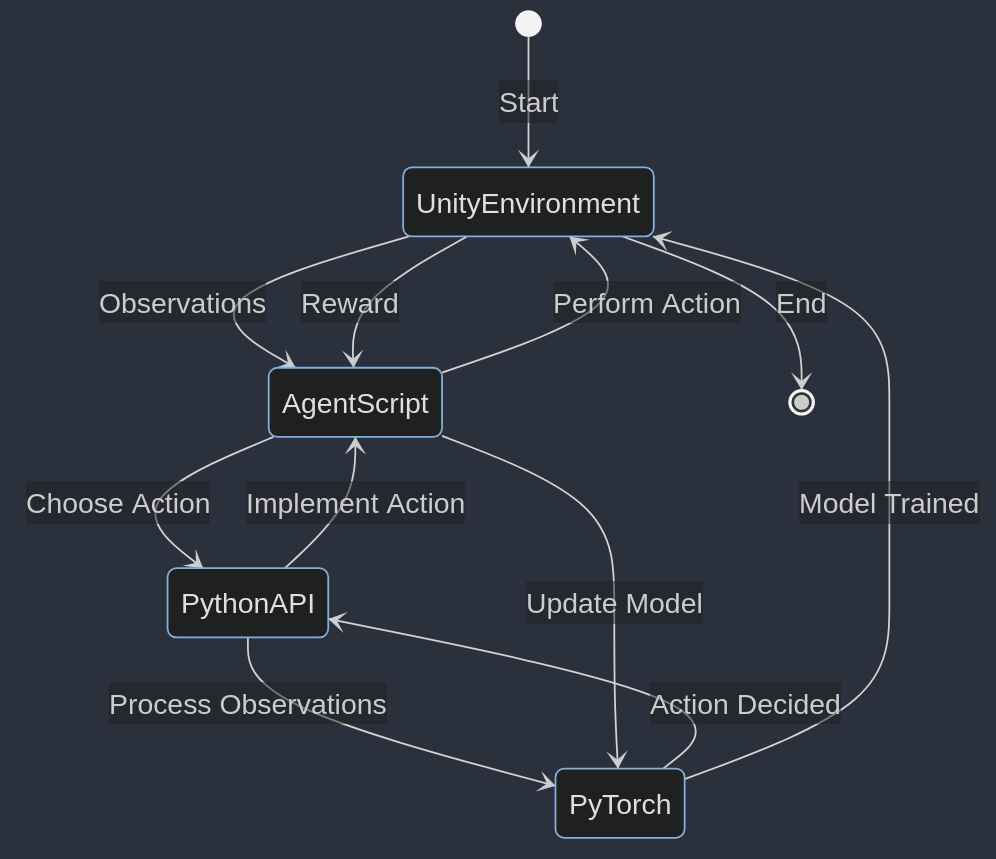
\includegraphics[width=0.5\textwidth]{Images/unity_mlagents.png}
    \caption{MLAgents Integration}\label{MLAgents_Integration}
\end{figure}



The technical instructions to setup MLAgents in Python and Unity can be found at 
\url{https://github.com/lipj01/AI-Kite-Control}

\section{The Environment}

The first step to this process is to create the environment, which the agent will use to train. In this case that will need to look something like a sailing game; it will have some form of water, a boat, a kite and a course. 
For any machine learning endeavor, especially one with such intricate physical dynamics, the choice of simulation environment is paramount. Not only does it provide the playground for our AI agent to learn and make mistakes safely, but it also serves as a litmus test for the robustness and realism of the designed model.

Given the myriad of choices available, the Unity game engine emerged as the most suitable platform. Beyond its reputation in gaming, 
The inherent support for mesh bodies, colliders, and a variety of joints made it an attractive option for simulating the kite-boat system, which comprised a complex dance of forces, and counterforces.
Unity is recognized for its potent physics engine, however for this project the use of Unity's physics engine will be kept to a minimum. Unity will be used primarily for its visual capabilities and the ability to run machine learning simulations. 

Central to our simulation is the depiction of water, the medium in which our boat will navigate. Here, the Unity HDRP Water System 16.0.3 [cite] came to the rescue. Bundled with Unity 2023.2.0b9 [cite], this water system provides a realistic representation of water with its undulating waves, refractions, and reflections. 
The alternative option to using Unity's water system was to model an entire particle fluid simulation, this would have had its advantages, however it would have been a lot more computationally expensive and would have taken a lot longer to implement. As this project was primarily focused on creating a RL algorithm for controlling a kiteboat it was decided that the Unity water system would be sufficient for this project.  

The boat part of the kiteboat had two main component scripts, the buoyancy and the rudder, allowing the boat to float and be steered. The implementation of Buoyancy and the rudder are discussed in more detail in section$~$\ref{sec:Boat}. The explanation of the kite model can be found in section$~$\ref{sec:Kite}.

Several assumptions were made for the initial model of the kiteboat. These assumptions were:
\begin{itemize}
    \item The Archimedes force is uniform across all submerged sections of the boat.
    \item The rudder forces of lift and drag could be aproximated to a torque applied about the rear of the boat.
    \item Once the boat is moving at a speed greater than 0.25m/s the lift and drag forces of the keel are equal to the downwind component of the kite's resultant force- essentially providing a non'slip condition.
    \item The kite is modeled as a symmetrical aerofoil, with constant lift and drag coefficients.
    \item Constant wind angle and laminar flow over the entire kite.
\end{itemize}
\subsection{Boat Model}\label{sec:Boat}
Buoyancy, the force that allows ships to float, was the first physical property to be addressed. Rooted in Archimedes' Principle, it dictates that the buoyant force exerted on a submerged body is equivalent to the weight of the fluid displaced by that body. In our Unity environment, the boat's hull, represented as a `mesh' with an associated `mesh collider', was divided into many small triangles or Voxels. These Voxels became the fundamental units for calculating buoyancy, allowing for a granular and realistic representation of the boat's interaction with water. This was achieved by first calculating the total Archimedes force (AF) of the entire boat using equation$~$\ref{archimedes}, followed by a local AF at each Voxel. The water level, y component, was then computed at each voxel's (x,z) coordinates to determine if it was above or below the surface. If below the surface the component of the AF was applied vertically at each voxel. This implementation can be viewed in the buoy.cs script in the project REF IN APENDIX.

\begin{equation}
    F_B = \rho_{w}gV
    \label{archimedes}
\end{equation}

While buoyancy ensures our boat doesn't sink, it's the rudder that grants it direction. The Rudder.cs script handles the implementation of the rudder and the keel. The equation for the torque applied about the rear of the boat is shown in equation$~$\ref{rudder_torque}. 

% the torque equation
% float turnForce = angle * boatForwardSpeed * rotationScale;
% boatRb.AddTorque(transform.up * turnForce);
\begin{equation}
    \tau = \alpha v R
    \label{rudder_torque}
\end{equation}

where $\tau$ is the torque, $\alpha$ is the angle of the rudder, $v$ is the speed of the boat and $R$ is the rotation scale.

\subsection{Kite Model}\label{sec:Kite}
The kite model was implemented using the kite.cs script. The kite was modeled as a symmetrical aerofoil, with constant lift and drag coefficients. The lift and drag forces were calculated using the equations shown in equation$~$\ref{lift} and equation$~$\ref{drag}.
\begin{equation}
    F_L = \rho C_L A \frac{v^2}{2} 
    \label{lift}
\end{equation}fixed at certain lengths, designed to permit movement across all rotational axis without any
\begin{equation}
    F_D = \rho v^2 C_D A \frac{v^2}{2} 
    \label{drag}
\end{equation}

where $F_L$ is the lift force, $F_D$ is the drag force, $\rho$ is the density of air, $C_L$ is the lift coefficient, $C_D$ is the drag coefficient, $A$ is the area of the kite and $v$ is the velocity of the kite relative to the wind.

In order to replicate the kite's mechanics and bar configuration, the model uses 4 configurable joints. These joints were fixed at certain lengths from the deck of the boat, designed to permit movement across all rotational axis without any `bounce' effect. This design enables the kite to descend or `fall' in conditions of low wind, mirroring real-world behavior where the kite may lose altitude but can be maneuvered back into position. To simulate the bar being pulled in, the lift and drag coefficients were increased, this has the effect of increasing the angle of attack of the kite.


\subsection{Collision Detection}
The Gilbert-Johnson-Keerthi (GJK)$~$\cite{gilbert88gjk} algorithm is a sophisticated method for collision detection between convex shapes. This algorithm was the approach taken to detect weather the kiteboat had reached the waypoint during training, and later, to work out if it had rounded the marks of the racecourse. The implementation of the GJK algorithm can be found in the GJK.cs script in the project REF IN APENDIX.
The GJK algorithm operates by iterative refinement of a simplex, which is a set of points that can define a line segment, triangle, or tetrahedron. The algorithm progresses by assessing whether the simplex contains the origin, which would imply an overlap between the two shapes. The initial direction d is determined by the normalized vector from mf1Pos to mf2Pos, constrained in the x-z plane by nullifying the y component, meaning the algorithm is only concerned with the horizontal plane.  

Within the GJK method, the Support function plays a pivotal role, calculating the Minkowski difference between the two shapes in a specified direction. This is achieved by finding the farthest points along that direction on both shapes and then subtracting them to obtain a single point in the Minkowski space.

The HandleSimplex function is a recursive strategy that adjusts the simplex and direction d based on whether the current simplex is a line or triangle. For a line, the LineCase function is invoked, and for a triangle, the TriangleCase is employed. These functions adjust the simplex and direction of search to move closer to the origin, if it is not already contained within the simplex.

% \subsection{Course Generation}

% \subsection{Mark Roundings}

\section{RL Implementation}\label{sec:RL_Implementation}

\subsection{The Agent Script}

\textbf{Controls}
In order to ensure the AI would be able to learn to sail the kiteboat a playable game version was created using arrow keys for the kite and `A' and `D' for the rudder.  

\subsection{Observations}

\subsection{Actions}



\subsection{Rewards}
Keep alive problem.

Diverse conditions

ciriculum style learning

\section{Initial Training}

\section{Optimization}

\subsection{Blue Crystal HPC}

The Blue Crystal HPC, operated by the University of Bristol, offers significant computational resources tailored for intensive tasks such as machine learning simulations, like.


To utilize Blue Crystal for MLAgents simulations, the following steps were undertaken:

\begin{itemize}
    \item \textbf{Access and Security:} Gained access to the university's HPC and set up SSH keys for secure communication.
    \item \textbf{File Preparation:} Built the .x86\_64 Unity build file and uploaded it, along with the necessary config file, to Google Drive.
    \item \textbf{Automation with Shell Script:} Developed a shell script to automate the process. This script:
    \begin{itemize}
        \item Retrieves the build files from Google Drive.
        \item Sets up a virtual environment on Blue Crystal.
        \item Installs the ML-Agents toolkit.
        \item Initiates the simulation.
        \item Upon completion, uploads the results back to Google Drive\textsuperscript{3}.
    \end{itemize}
\end{itemize}

Useful commands for working with Blue Crystal:

\begin{itemize}
    \item \textbf{sbatch:} Submits a job to the queue.
    \item \textbf{sacct:} Checks the status of a job.
    \item \textbf{scancel:} Cancels a job.
\end{itemize}

Parallelization and Optimization:

Initially, a single node on Blue Crystal was employed to run the simulation. This node with 28 CPUs was responsible for both hosting the environment and executing the model. However, Blue Crystal's architecture allows for more advanced parallelization strategies. Distributing the simulation across multiple nodes can enhance efficiency. Additionally, offloading the ML-Agents toolkit to a GPU core can further accelerate the learning process.

However, it's worth noting that the demand for GPUs on Blue Crystal is high. For tasks that don't necessitate the power of GPUs, relying on CPUs, even if they take longer, is a practical choice given the limited GPU availability.





%=========================================================